 
In this chapter, the context of this thesis and the general problems it faces are introduced. The objective of this chapter is to give a brief introduction to  different domains and concepts in which our work takes place and used throughout this document.
This includes an overview of the generative programming development process, the main concepts for tuning and testing configurable code generators, and the main challenges they raise.

 %It aims at providing a better understanding of the background and context in which our work takes place, as well as the terminology and concepts presented in the next chapters.

The chapter is structured as follows: 

In Section \ref{bg:Diversity in software engineering}, we present the problem of software diversity and hardware heterogeneity carried out by the continuous innovation in science and technology.

Section \ref{sec:FROM} aims at providing a better understanding of the generative programming concept that is increasingly applied to ease software development. We present the different steps of automatic code generation involved during software development as well the different stakeholders and their roles in testing generators. We highlight then, the main activities that the software developer goes through from the software design until the release of the final software product.

Section \ref{bg:Testing code generators} gives an overview of the different types of code generators used in the literature and we show the complexity of testing code generators.. 

Similarly, in Section \ref{bg:Compilers auto-tuning}, we describe some compiler optimizations and we illustrate the compiler auto-tuning complexity by presenting the different challenges that this task is posing.

Finally, we conclude by providing a summary, in Section \ref{bg:Summary: Testing and optimization challenges}, of the main challenges we have identified regarding code generators testing and compiler tuning.

\section{Diversity in software engineering}
\label{bg:Diversity in software engineering}
%context
The history of software development shows a continuous increase of complexity in several aspects of the software development process. This complexity is highly correlated with the actual technological advancement in the software industry as more and more heterogeneous devices are introduced in the market~\cite{betz2011improving}. 
Generally, heterogeneity may occur in terms of different system complexities, diverse programming languages and platforms, types of systems, development processes and distribution among development sites\cite{ghazi2015heterogeneous}.
%System heterogeneity we are discussing in this thesis is the software and hardware diversity.
System heterogeneity is often led by software and hardware diversity.
Diversity emerges as a critical concern that spans all activities in software engineering, from design to operation\cite{acher2014software}. It appears in different areas such as mobile and web development\cite{doukas2013compose}, security\cite{allier2015multitier}, etc.

However, software and hardware diversity leads to a greater risk for system failures due to the continuous change in configurations and system specifications.
As a matter of a fact, effectively developing software artifacts for multiple target platforms and hardware technologies is then becoming increasingly important.
Furthermore, the increasing relevance of software in general and the higher demand in quality and performance contribute to the complexity of software development.

In this background introduction, we discuss two different dimensions of diversity: (1) software diversity and (2) hardware heterogeneity.

%The history of software development shows a continuous increase of complexity in several aspects of the software development process~\cite{betz2011improving}. 
%Diversity
 
 
%problem
%Furthermore, the increasing relevance of software in general and the higher demand in quality and performance contribute to the complexity of software development. 
%Today, softwares and services are running everywhere. These services are running on top of heterogeneous software and hardware platforms.
\subsection{Hardware heterogeneity}
Modern software systems rely nowadays on a highly heterogeneous and dynamic interconnection of devices that provide a wide diversity of capabilities and services to the end users.
These heterogeneous services run in different environments ranging from cloud servers to resource-constrained devices.
Hardware heterogeneity comes from the continuous innovation of hardware technologies to support new system configurations and architectural design (e.g., addition of new features, a change in the processor architecture, new hardware is made available, etc). 
For example, until February 2016\footnote{\url{https://arstechnica.com/information-technology/2016/02/moores-law-really-is-dead-this-time/}}, the increase in capacity of microprocessors has followed the famous Moore's law\footnote{\url{https://en.wikipedia.org/wiki/Moore\%27s_law}} for Intel processors. Indeed, the number of components (transistors) that can be fitted onto a chip doubles every two years, increasing the performance and energy efficiency.
For instance, Intel Core 2 Duo processor was introduced in 2006 with 291 millions of transistors and 2.93 GHz clock speed. Two years later, Intel has introduced the Core 2 Quad processors which came up with 2.66 GHz clock speed and the double number of transistors introduced in 2006 with 582 millions of transistors.

In the last years, modern processors becomes more and more heterogeneous, using more than one kind of processor or cores, called "co-processors". The CPU can even use different instruction set architectures (ISA), where the main processor has one and the rest have another, usually a very different architecture. Operations performed by the co-processor may be floating point arithmetic, graphics, signal processing, string processing, encryption or I/O Interfacing with peripheral devices. 
As an example, the ARM big.Little processor architecture\footnote{\url{https://en.wikipedia.org/wiki/ARM_big.LITTLE}} released in 2011 (see Figure \ref{fig:cortex}), is a power-optimization technology where high-performance ARM CPU cores are combined with the most efficient ARM CPU cores to deliver peak-performance capacity, higher sustained performance, and increased parallel processing performance, at significantly lower average power. It can save 75\% of CPU energy and can increase performance by 40\% in highly threaded workloads.
The intention of this architecture is to create a multi-core processor that can adjust better to dynamic computing needs.
Threads with high priority or computational intensity can in this case be allocated to the "Big" cores while threads with less priority or less computational intensity, such as background tasks, can be performed by the "Little" cores. This model has been implemented in the Samsung Exynos 5 Octa in 2013\footnote{\url{http://www.embedded.com/electronics-news/4419448/Benchmarking-ARM-s-big-little-architecture}}.


\begin{figure}[h]
	\center
	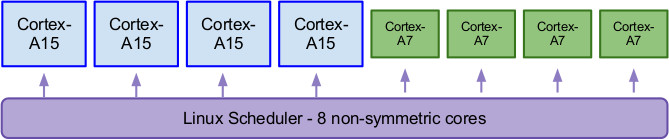
\includegraphics[scale=0.7]{Background/fig/cortex.jpg}
	\caption{ARM Big.Little heterogeneous multi-processing}
	\label{fig:cortex}
\end{figure}


Given the complexity of new emerging processors architecture (x86, x64, multi-core, etc) and CPU manufacturers such as ARM, AMD and Intel, some of the questions that developers have to answer when facing hardware heterogeneity: 
Is it easy to deliver satisfactory levels of performance on modern processors? How is it possible to produce machine code that can exploit efficiently the continuous hardware changes? 





%Which optimizations are applied by compiler users in order to satisfy  the non-functional properties of a broad range of programs and hardware architectures such as energy consumption, execution time, etc. 


%end 


%Model-Driven Software Engineering and generative programming techniques to provide a new integrated software engineering approach which enables the advanced exploitation of the full range of diversity and specificity of the future computing continuum

%Diversity increases system complexity and leads to a greater risk for system failures. Efficient validation and verification methods are, thus, essential to guarantee qualities of diverse systems, such as security, consistency, correctness or performance

\subsection{Software diversity}
\label{sec:Software diversity}
In today's software systems, different software variants are typically developed simultaneously to address a wide range of application contexts and customer requirements\cite{schaefer2012software}. 
Therefore, software is built using different approaches and languages, depending on the application domain.

In the literature, Baudry et al.\cite{baudry2015multiple} and Schaefer et al.\cite{schaefer2012software} have presented an exhaustive overview of the multiple facets of software diversity in software engineering. 
According to their study, software diversity can emerge in different types and dimensions such as diversity of operating systems, programming languages, data structures, components, execution environments, etc. 
Like all modern software systems, softwares have to be adapted to address changing requirements over time supporting system evolution, technology and market needs like considering new software platforms, new languages, new customer choices, etc.

In order to understand the skills and capabilities required to develop softwares on top of different classes of devices and application domains, we queried a popular open-source repository \textit{GitHub} to evaluate the diversity of existing programming languages.  
The following sets of keywords were used: \textit{1) Cloud:} server with virtually unlimited resources, \textit{2) Microcontroller:} resource constrained node (few KB RAM, few MHz),  \textit{3) Mobile:} an intermediate node, typically a smartphone,  \textit{4) Internet of Things:} Internet-enabled devices,  \textit{5) Cyber Physical System}, and  \textit{6) Embedded systems}, as a large and important part of the service implementations will run as close as possible to physical world, embedded into sensors, devices and gateways.

\begin{figure}[h]
	\center
	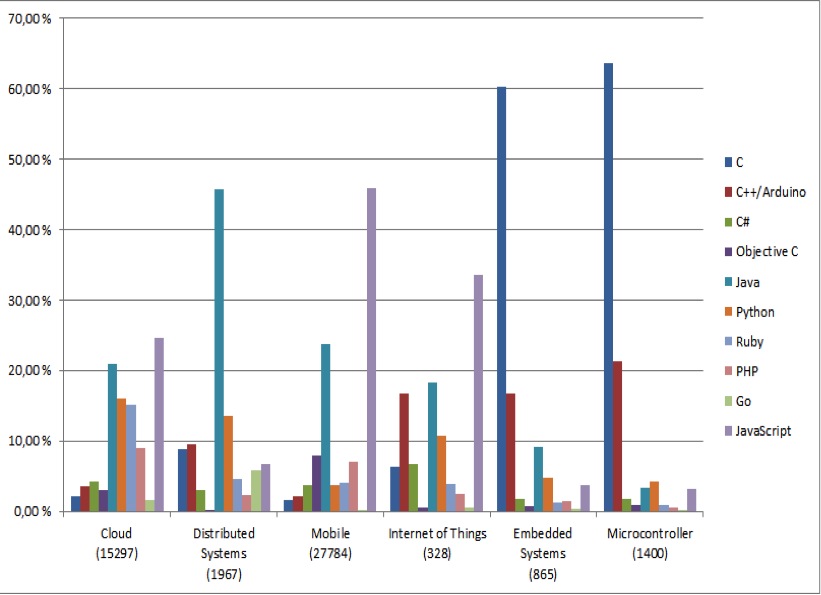
\includegraphics[scale=1.]{Background/fig/github}
	\caption{Popularity of 10 programming languages for the different areas related to software development}
	\label{fig:github}
\end{figure}

Figure \ref{fig:github} presents the results of those queries. The queried keywords are presented on the x-axis together with the number of matches for that keyword. For each keyword, the y-axis represents the popularity (in per cent of the total number of matches) of each of the 10 most popular programming languages that we encountered.


This simple study indicates that no programming language is popular across the different areas. A general trend indicates that Java and JavaScript (and to some extent, Python and Ruby) are popular in cloud and mobile, whereas C (and to some extent, C++) is a clear choice for developers targeting embedded and microcontroller-based systems. Other languages do not score more 10\% for any of the keywords. 
For all keywords except Cloud , the combined popularity of Java, JavaScript and C/C++ (i.e, the sum
of the percentages) is above 70\%. For Cloud, we observe a large use of Python, Ruby also being very popular, so the combined popularity of Java, JavaScript and C/C++ is only 50\%. It is also worth noticing that the most popular language for a given keyword scores very poorly (less than 5\%) for at least another keyword. While it might appear that a combination of C/C++, JavaScript and Java should be able to cover all the areas, in practice it does not exclude the need for other programming languages. For example, the Fibaro Home Center 2 (a gateway for home automation based on the Z-Wave protocol) uses Lua as scripting language to define automation rules. Another example is the BlueGiga BlueTooth Smart Module, which can be scripted using BGScript, a proprietary scripting language. This shows that each part of an infrastructure might require the use of a niche language, middleware or library to be exploited to its full potential.


In summary, the variation of programming languages for the different kinds of devices and application domains induces a high \textit{software diversity}. Accordingly, we propose the following definition of software diversity in the context of this thesis: 
\textit{Software diversity is the generation or implementation of the same program specification in different ways/manners in order to satisfy one or more diversity dimension such as the diversity of programming languages, execution environments, functionalities, etc. }
		
%We define as well the term \textbf{"software family"} to categorize these diverse programs that share commonalities. 

%The key concept of code generators is to produce code in a general-purpose language, such as Java or C++, that can be compiled and executed. Target execution platforms of the generated code are heterogeneous and diverse.



\subsection{Matching software diversity to heterogeneous hardware: the marriage}
\subsubsection{Challenges}
The hardware and software communities are both facing significant change and major challenges. Figure \ref{fig:marriage} shows an overview of the challenges that both communities are facing. In fact, hardware and software are pulling us in opposite directions. 

\begin{figure}[h]
	\center
	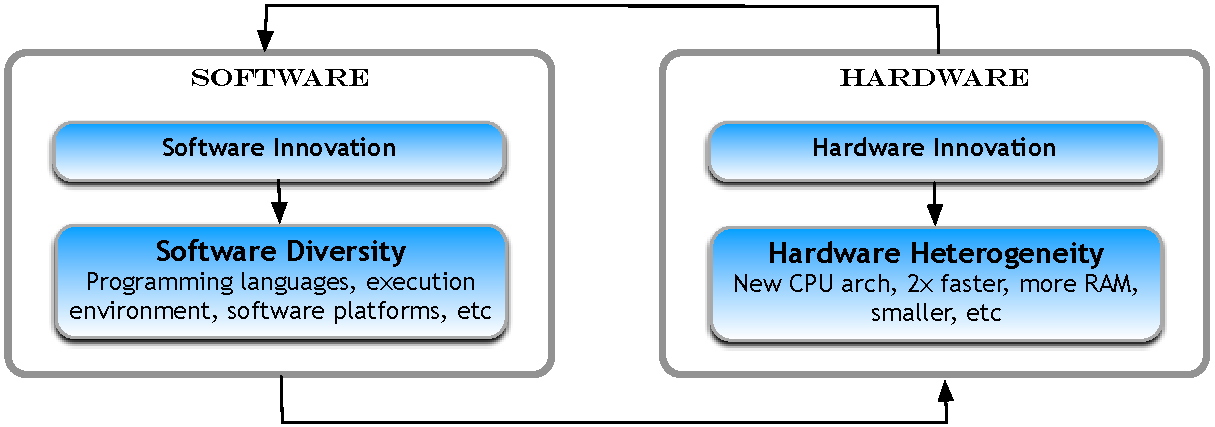
\includegraphics[scale=0.65]{Background/fig/marriage}
	\caption{Matching software to hardware}
	\label{fig:marriage}
\end{figure}


On the one hand, software is facing challenges of a similar magnitude, with major changes in the way software is deployed, is sold, and interacts with hardware. 
Software diversity, as discussed in Section \ref{sec:Software diversity}, is driven by software innovation, driving the software development toward highly configurable and complex systems. This complexity is carried by the huge diversity of software technologies, customer configurations, execution environments, programming languages, etc. This explosion of configurations that software is facing makes the activity of testing and validation very difficult and time consuming. 
As a consequence, softwares become higher and higher level, managing complexity and gluing lot of pieces together to give programmers the right abstraction for how things really work and how the data is really represented. 


On the other hand, hardware is exposing us to more low level details and heterogeneity due to the continuous hardware innovation. 
Hardware innovation offer us energy efficiency, performance improvement but exposes a lot of complexity for software engineers and developers.
For example, in \cite{he2010computer}, authors argue that system software is not ready for this heterogeneity and cannot fully benefit from new hardware advances such as multi-core and many-core processors. Although multi-core processors have been used in everyday life, we still do not know how to best organize and use them. 
Meanwhile, hardware specialization for every single application is not a sustainable way of building chips.
%So, what the software community can do to address/deal with devices heterogeneity? How hardware innovation can be exploited in the software?

%\paragraph{So how can we match software diversity to heterogeneous hardware?}~\\ 
\subsubsection{Mapping software to hardware}
\label{Mapping software to hardware}
Matching software to hardware is ensured by the efficient translation of the high-level software programs into a machine code that better exploit the hardware changes (relation 1 in Figure \ref{fig:marriage}). This is exactly what a compiler is intended to do.

\paragraph{Configuring existing compilers}~\\ 
Well, gone are the days where we used to write the assembly code by hand and from scratch. Now, it is up to the compilers to handle this heterogeneity and to efficiently generate and optimize the code for a particular microprocessor. 

As shown in Figure \ref{fig:compilers}, a compiler is typically divided into two parts, a front-end and a back-end. The compiler front-end verifies the syntax and semantics and analyzes the source code to build an internal representation of the program, called the intermediate representation or IR. For example, the GNU Compiler Collection (GCC) and LLVM support many front-ends with programming languages such as C, C++, Objective-C, Objective-C++, Fortran, Java, Ada, and Go among others. The compiler back-end generates the target-dependent assembly code and performs optimizations for the target hardware architecture. Typically, the output of a back-end is a machine code specialized for a particular processor and operating system (e.g., ARM, Sparc processors, etc).
As consequence, people who are writing compilers have to continuously enhance the way these executables are produced by releasing new compiler versions to support new hardware changes (i.e., introducing new optimization flags, instruction sets, etc.). 
\begin{figure}[h]
	\center
	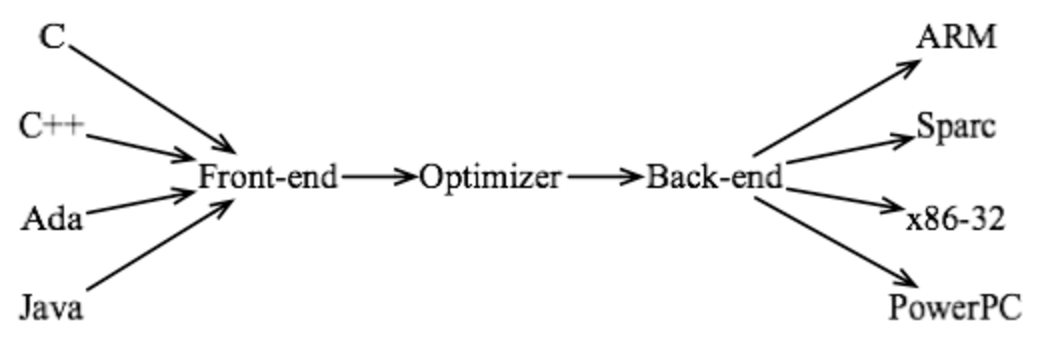
\includegraphics[scale=0.65]{Background/fig/compilers}
	\caption{Compiler architecture}
	\label{fig:compilers}
\end{figure}

Let's take the GCC example. GCC is able to generate code automatically for approximately \textbf{more than 40 different processor architectures}. Hence, GCC becomes highly configurable, allowing the compiler user to enable multiple flags to customize the code generation. For instance, one important compiler flag is \textit{-march}. It tells the compiler what code it should produce for the system's processor architecture (or arch); it tells GCC that it should produce code for a certain kind of CPU. Using \textit{-march=native} enables all the optimization flags that are applicable for the native system's CPU, with all its capabilities, features, instruction sets, and so on. There exits many other configuration options for the target CPU like \textit{--with-arch=i7}, \textit{--with-cpu=corei7}, etc.
Generally, each time a new family of processors is released, compiler developers release a new compiler version with more sophisticated configuration options for the target platform. For example, old compilers produce only 32-bit programs. These programs still run on new 64-bit computers, but they may not exploit all processor capabilities (e.g. they will not use the new instructions that are offered by x64 CPU architecture). For instance, the current x86-64 assembly language can still perform arithmetic operations on 32-bit registers using instructions like addl, subl, andl, orl, etc, with the l standing for "long", which is 4 bytes/32 bits. 64-bit arthimetic is done with addq, subq, andq, orq, etc, with q standing for "quadword", which is 8 bytes/64 bits.

Another example is that compilers need to support parallelism. In fact, we can see that modern computers today can do many things at once and modern CPUs becomes highly parallel processors with different levels of parallelism (e.g., the ARM Big.Little in Figure \ref{fig:cortex}). We find parallelism everywhere from the parallel execution units in a CPU core, up to the SIMD (Single Instruction, Multiple Data) instruction set and the parallel execution of multiple threads.  One of the commonly applied optimizations by modern compilers in parallel computing is vectorization. It constitutes the process of converting an algorithm from a scalar implementation, which processes a single pair of operands at a time, to a vector implementation, which processes one operation on multiple pairs of operands at once (series of adjacent values).
Programmers can exploit vectorization using compilers to speedup certain parts of their code. One hot research topic in computer science is the search for methods of automatic vectorization\cite{nuzman2006auto}: seeking methods that would allow a compiler to convert scalar algorithms into vectorized algorithms without human intervention.


Therefore, to cope with the heterogeneous hardware platforms, software developers use these highly configurable compilers (for compiled languages such as C or C++) in order to efficiently compile their high-level source code programs and execute them on top of a board range of platforms and processors. 


\paragraph{Masking hardware heterogeneity}~\\ 
Sometimes, software developers try to avoid the hardware heterogeneity. Thus, they use for example managed languages such as JAVA, Scala, C\#, etc to favor software portability. Instead of compiling to native machine instruction set, these languages are compiled into an intermediate language or IL, which is similar to a binary assembly language. These instructions are executed by a JVM, or by .NET's CLR virtual machine, which effectively translates them to native binary instructions specific to the CPU architecture and/or OS of the machine.
By using managed code and compiling in this managed execution environment, memory management such as a garbage collector, type safety checking, and destruction of unneeded objects are handled internally within this sandbox runtime environment. Thus, developers focus on the business logic of applications to provide more secure and stable software without taking too much care of the hardware heterogeneity.
However, using managed languages has drawbacks. It includes slower startup speed (the managed code must be JIT compiled by the VM). It can also be slower than native code and generally more greedy in terms of system resources. 
For example, we can see in Figure \ref{fig:github}, that the C language is the most widely used programming language in the context of embedded systems\footnote{\url{http://www.eetimes.com/author.asp?doc_id=1323907}} where the system is really resource-constrained. Contrarily to managed languages, C utilizes the hardware to its maximum by multi-processing and multi-threading APIs provided by POSIX. It also controls the memory management and uses less memory (which allows more freedom on memory management compared to the use of garbage collector).   


\paragraph{Building new DSLs and compilers}~\\ 
An alternative approach for matching software to hardware is to build new languages and compilers for a specific domain from scratch. 
For example, Hou et al.\cite{hou2010spap} have presented a container-based programming language for heterogeneous many-core systems. This DSL allows programmers to write unified programs that are able to run efficiently on heterogeneous processors. To map this DSL to such hardware processors, they provide a set of compilers and runtime environments for the x86 CPUs
and CUDA GPUs. Similarly, Chafi et al.\cite{chafi2010language,chafi2011domain} proposed leveraging DSLs to map high-level application code to heterogeneous devices. Results show that the presented DSL can achieve high performance on heterogeneous parallel hardware with no modification required to the source code. They compared this language performance to MATLAB code and they showed that it outperformed it in nearly all cases.

%In contrast, devices in turn, may impose the support of specific programming languages (relation 2 in Figure \ref{fig:marriage}). 
%In mobile development for example, Java is needed to implement Android applications and Objective-C is needed to develop iOS products. This means that developers need to create multiple clients in this heterogeneous environment. 
%We can see also that C/C++ are the most used languages for targeting embedded systems.

%Well, it's like this. Every language is created with a single target platform in mind ( except haXe of course, it can target multiple platforms). For example, Java is compiled into Java bytecode which is executed in the Java Platform ( Java Runtime Library). C/C++ is used to built  applications executed by the OS. So, the target platform of C/C++ is a specific OS. C# is built for the Microsoft .NET framework. Javascript is built for the web platform.
%But, the problem with this is that each platform has its own language tied to it, so it is very difficult to write for different platforms as you need to program in different languages. Also, it becomes difficult to combine platforms together.

%This is where haXe steps in to show us the way. To quote from the haXe website :
%IF YOU COULD ONLY LEARN ONE PROGRAMMING LANGUAGE, HAXE WOULD BE IT.
%IT'S UNIVERSAL. IT'S POWERFUL. IT'S EASY-TO-USE.

 

%which is big problem for both communities
%we need a marriage between hardware and software



%to handle hardware hetergenouty is parallalism ubiquity and differentiation


 %abstract, choose, and exploit hardware heterogeneity providing computational power at low energy consumption levels.

%For example, although Android provides Java syntax, it uses its own Google libraries and creates byte code that will not run on the standard JVM (Java Virtual Machine). This means that consumers are carrying devices that support different programming languages and developers will usually need to create multiple clients in this heterogeneous environment.

In short, hardware heterogeneity raises many challenges for the software community that need to create or deal with highly configurable code generators (i.e. Compilers) to truly take advantage of the new chip with more advanced optimizations for the new hardware settings.

\section{From classical software development to generative programming}
\label{sec:FROM} 
In comparison to the classical approach where software development was carried out manually, today’s modern software development requires more automatic and flexible approaches to face the continuous innovation in industry production, as described in the previous sections.
Hence, more generic tools, methods and techniques are applied in order to keep the software development process as easy as possible for testing and maintenance and to handle the different requirements in a satisfyingly and efficient manner.
%GP
As a consequence, generative programming (GP) techniques are increasingly applied to automatically generate and reuse software artifacts.
%GP definition
\begin{mydef}[\textbf{Generative programming}]
		Generative programming is a software engineering paradigm based on modeling software families such that, given a particular requirements specification, a highly customized and optimized intermediate or end-product can be automatically manufactured on demand from elementary, reusable implementation components by means of configuration knowledge~\cite{Czarnecki:2000:GPM:345203}.
\end{mydef}

This paradigm offers the promise of moving from "one-of-a-kind" software systems to the semi-automated manufacture of wide diversity of software.

%figure
Generative software engineering consists on using higher-level programming techniques such as meta-programming, modeling, DSL, etc. in order to provide a new integrated software engineering approach which enables the advanced exploitation of the different dimensions of software diversity and automatically generate efficient code for the target software platform. 

In principle, a software development process can be seen as a mapping between a problem space and a solution space~\cite{czarnecki2005overview} (see Figure \ref{fig:GDM}). 

%problem space
\textbf{The problem space} is a set of domain-specific abstractions that can be used by application engineers to express their needs and specify the desired system behavior. This space is generally defined  as DSLs or high-level models. 

%solution space
\textbf{The solution space} consists of a set of implementation components, which can be composed to create system implementations (for example, the generation of platform-specific software components written using general-purpose languages such as Java, c++, etc).

%mapping
\textbf{The configuration knowledge} constitutes the mapping between both spaces. It takes a specification as input and returns the corresponding implementation as output. It defines the construction rules (i.e., the translation rules to apply in order to translate the input model/program into specific implementation components) and optimizations (i.e., optimization can be applied during code generation to enhance some of the non-functional properties such as execution speed). It defines also the dependencies and settings among the domain specific concepts and features.

\begin{figure}[h]
	\center
	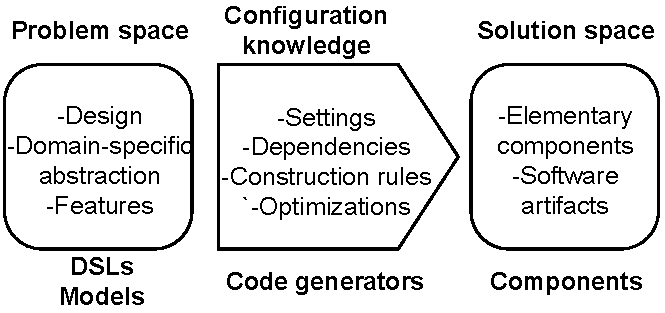
\includegraphics[scale=0.65]{Background/fig/GDM.pdf}
	\caption{Generative programming concept}
	\label{fig:GDM}
\end{figure}
%GP advantages
These schema integrates several powerful concepts from model driven engineering, such as domain-specific languages, feature modeling, and code generators.

Some commonly benefits of such software engineering process are:
\begin{itemize}
\item It reduces the amount of re-engineering/maintenance caused by specification requirements
\item It facilitates the reuse of components/parts of the system
\item It increases the decomposition and modularization of the system
\item It handles the heterogeneity of target software platforms by automatically generating code
\end{itemize}

An example of generative programming application is the use of Software Product Lines (SPL)\cite{schaefer2012software}.
SPL-based software diversity is often coupled to generative programming techniques\cite{Czarnecki:2000:GPM:345203} that enable the automatic production of source code from variability models. This technique implies the use of automatic code generators to generate code that satisfies user requirements (SPL models).
This technique enables one to manage a set of related features to build diverse products in a specific domain. Thus, this solution is able to control software diversity by handling the diversity of requirements such as user requirements or environmental constraints or changes. 

%In the following section, we present a general overview of the complete software development tool chain and the main actors that are involved from design time to runtime.


\subsection{Overview of the generative software development process}
The process of generative software development involves many different technologies. In this section, we describe in more details the different activities and stakeholders involved to automatically transform the high-level system specifications into executable programs and that from design time to runtime.
\begin{figure}[h]
	\center
	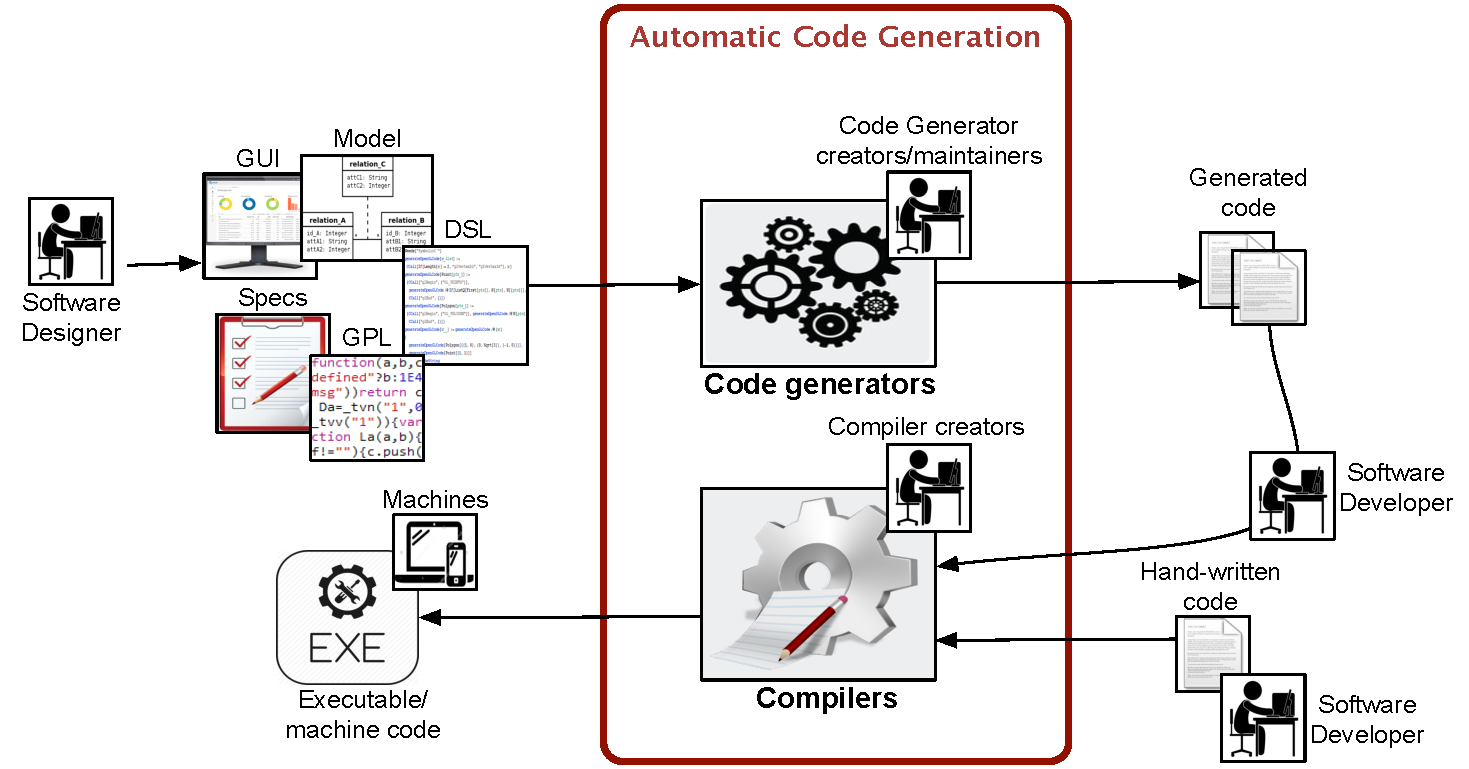
\includegraphics[scale=0.65]{Background/fig/background_overview2.pdf}
	\caption{Overview of the generative software development process}
	\label{fig:background_overview2}
\end{figure}
%\subsection{Automatic code generation}
Figure \ref{fig:background_overview2} gives an overview of the generative software development as we see in the context of this thesis. We distinguish four main tasks necessary for ensuring the automatic code generation: 



\begin{enumerate}
	\item \textbf{\textit{Software design:}} 
	As part of the generative programming process, the first step consists on representing the system behavior. 
	%Software design/behavior is the input program for the code generators. 
	On the input side we can either use code as the input or an abstract form that represents the design. It depends on the type of the code generator and on the input source program it requires. These programs can range from a formal specification of the system behavior to abstract models that represents the business logic.
	For example, software designers can define, at design time, software’s behavior using for example Domain-Specific Models (DSMs).
	A DSM, as an example, is a system of abstractions that describes selected aspects of a sphere of knowledge and real-world concepts pertinent to the domain that need to be modeled in software. These models are specified using high-level abstract languages (i.e., DSLs). %Domain-specific languages (DSLs) improve programmer productivity by providing high-level abstractions for the development of applications in a particular domain. Furthermore, software design can be provided as GUIs, GPLs, Models, etc.
	
	\item \textbf{\textit{Code generation:}} 
	Code generation is the technique of building code using programs. The common feature of the generator is to produce code that the software developer would otherwise write by hand.
	%There is no one style of code generation. 
	Generators are generally seen as a black box which requires as input a program and generate as output a source code for a specific target software platform/language. %Generators can work on the command line or using a GUI. 
	Code generation can build code for one or more target language, once or multiple times. There are different varieties of code generation aspects and it highly depends on the type of the input programs described in the previous step. 
	%Code generation techniques depends generally on these inputs.  
	For example, code generator developers use model-driven engineering techniques in order to automatically generate code. Thus, instead of focusing their efforts on constructing code, they build models and, in particular, create model transformations that transform these models into new models or code. Thus, the code generation process start by taking the previously defined specification to translate a model to an implementation in a target language. We will see in Section \ref{bg:Types of code generators} the different types of code generators.
	
	
	%In general, there are two main categories of Automatic code generation: passive or active.  Passive code generators build the code once, then have nothing more to do with the code.  It is up to the discretion of the user as to how to update and maintain the code.  Active code generators, on the other hand, keep track of the code during its lifecycle.  Active code generators are run on code multiple times during the lifecycle.  With Active Code generators, there is code you can modify, and code that should only be modified by the code generator.  Code generators can be further classified into code mungers, inline code expanders, mixed code generators, partial class generators, tier generators and domain languages\cite{fertalj2008source}. 
	
	\item \textbf{\textit{Software development:}}
	Software development may be divided into two main parts. On the one hand, software developers may follow the two previous steps in order to automatically generate code for a specific target software platform. In this case, they use to edit the system specification described in the first step (at a high level) and use to re-generate code each time needed by calling a specific generator. In some cases, generated code can even be edited by the end software developers. This task depends on the complexity of the generated code. Sometimes, it requires the help of domain experts who have enough expertise and knowledge to easily update and maintain the automatically generated code. On the other hand, they may manually implement the source code from scratch without going through any abstractions or code generation aspects. In this case, they may integrate the manually-written code with the automatically generated in order to deliver the final software product.
	
	\item \textbf{\textit{Compilation:}}
	Once code is generated or implemented, a classical compiler is used (if needed) to translate the generated code into an executable one. This translation depends on the target hardware platforms and it is up to the software developer to select the adequate compiler to use. Compilers are needed to target heterogeneous and diverse kinds of hardware architectures and devices. 
	As an example, cross compilers may be used to create executable code for a platform other than the one on which the compiler is running. In case the generated code needs to run on different machines/devices, the software developer needs to use different compilers for each target software platform and deploy the generated executables within different machines which is a tedious and time-consuming task.
	
\end{enumerate} 


\subsection{Automatic code generation in GP: a highly configurable process}
Among the main advantages that GP offers, is the automatic code generation, highlighted with red box in Figure \ref{fig:background_overview2}. Automatic code generation emerges in two principal aspects: 
\begin{enumerate}
	\item The use of code generators to cope with the software diversity and produce code for a range of software languages and platforms. GP provides an abstraction layer that hide the technical and implementation details. Instead, it relies on code generators to automate the code transformation process and to target a broad range of software platforms.
	\item The use of compilers to cope with the hardware heterogeneity, as discussed in Section \ref{Mapping software to hardware}. Compilers are needed to automatically transform the generated or manually written code to machine code that will be running on the target hardware.
\end{enumerate}

Both, compilers and code generators, are responsible for the automatic code generation in GP. 
In fact, we realize that this process is highly configurable. 

Compilers, on the one hand, become very user-friendly, letting the user to easily introduce optimizations and customize the machine code to fit with target hardware settings.
As an example, Table \ref{iccgccllvm} depicts the number of optimizations available in three popular compilers. The user can configure the compiler by selecting one of the $2^{n}$ possible optimizations sequences, where $n$ is the number of optimizations available in the compiler. We can see that the configuration space is very large. 

\begin{table}[h]
	\centering
	\caption{Number of optimizations in LLVM, GCC, and ICC}
	\label{my-label}
	\begin{tabular}{|c|c|c|}
		\hline
		\textbf{Compiler} & \textbf{\#Optimizations} & \textbf{\#Combinations} \\ \hline
		\textbf{LLVM}     & 100    & $2^{100}$                                 \\ \hline
		\textbf{GCC}      & 250    & $2^{250}$                                 \\ \hline
		\textbf{ICC}      & 75     & $2^{75}$                                 \\ \hline
	\end{tabular}
	\label{iccgccllvm}
\end{table}

On the other hand, code generators offer the possibility to customize the generated code for the target software platform. Code generators are less configurable than compilers because they do not interact with the hardware and they provide only general passes necessary for building the software artifact (e.g., select the target programming language, platform settings, libraries, etc.).
As an example, JHipster\footnote{https://jhipster.github.io/} is a concrete example of generative programming application in industry. JHipster is an application generator based on YO generator which provides tools to generate quickly modern web applications using Java stack on the server side (using Spring Boot) and a responsive Web front-end on the client side (with AngularJS and Bootstrap).
The generated web application can be quite different from one user to another. It really depends on the options/choices selected by the user to build a configured application. The selected parameter values will configure the way the JHipster code generators will produce code. 
For example, Figure \ref{fig:jhipster} shows a feature model of some configuration examples that the user would select. When building the applications, the user may select the database type he would generate, the Java version, the network protocol, etc. 
Using this feature model, \textbf{more than 10k diverse architecture types} of project can be selected which means that 10k program variants may be generated depending on the different criteria.
Whatever configuration selected by the user, the application behavior will not change and the generated application will share a similar architecture and fundamental code-base.
Among the main contributions of this thesis is to evaluate the impact of applied configurations during code transformation/optimization (by whether code generators or compilers) on the resource usage requirements.
\begin{figure}[h]
	\center
	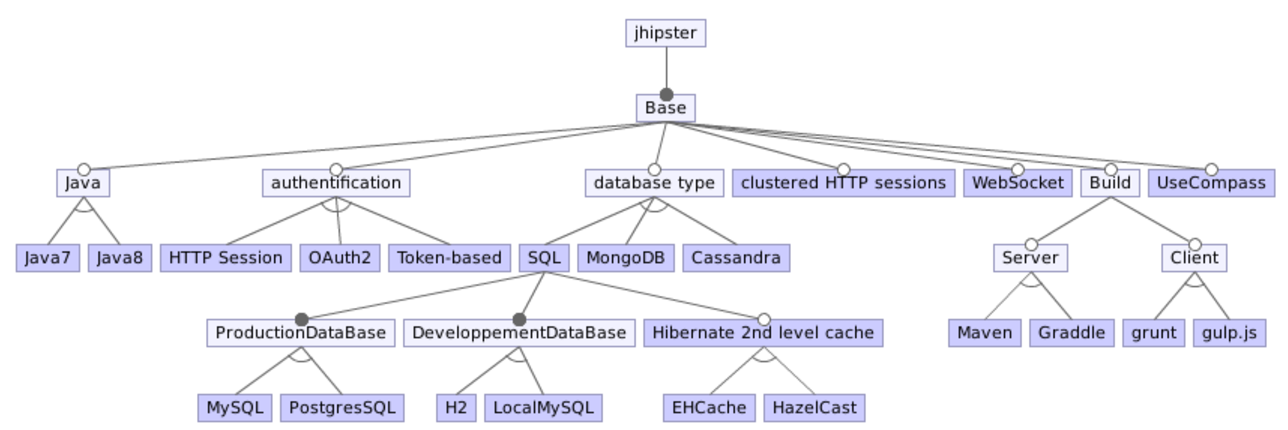
\includegraphics[scale=0.65]{Background/fig/jhipster}
	\caption{Example of JHipster feature model}
	\label{fig:jhipster}
\end{figure}

Well, we can see that both generators are highly configurable. However, in practice, code generators are less used in industry compared to compilers. First, because compilers are required for machine code production and optimization. Then, they are rigorously tested (by compiler suppliers) and the users of popular compilers such as GCC or LLVM have enough experience and confidence on the correct translation of the code. 
Code generators on the other side, are less used because users do not have enough experience with the code generator and need to gain confidence on their correct functioning by rigorously testing them. The code generator user can gain confidence in the tool only if he run his own tests.

In summary, the generative software development faces two major challenges. On the one hand, compilers become highly configurable and widely used. Thus, they need to be efficiently tuned in order to produce high quality machine code. On the other hand, since code generators become essential actors in GP, they need to be rigorously tested in order to provide evidence to the users to trust them and continue using them for production code generation.

We describe in the next section the main stakeholders involved in the automatic code generation process of GP and their roles for validating this process.


\subsection{Stakeholders and their roles for testing and tuning generators}
\begin{figure}[h]
	\center
	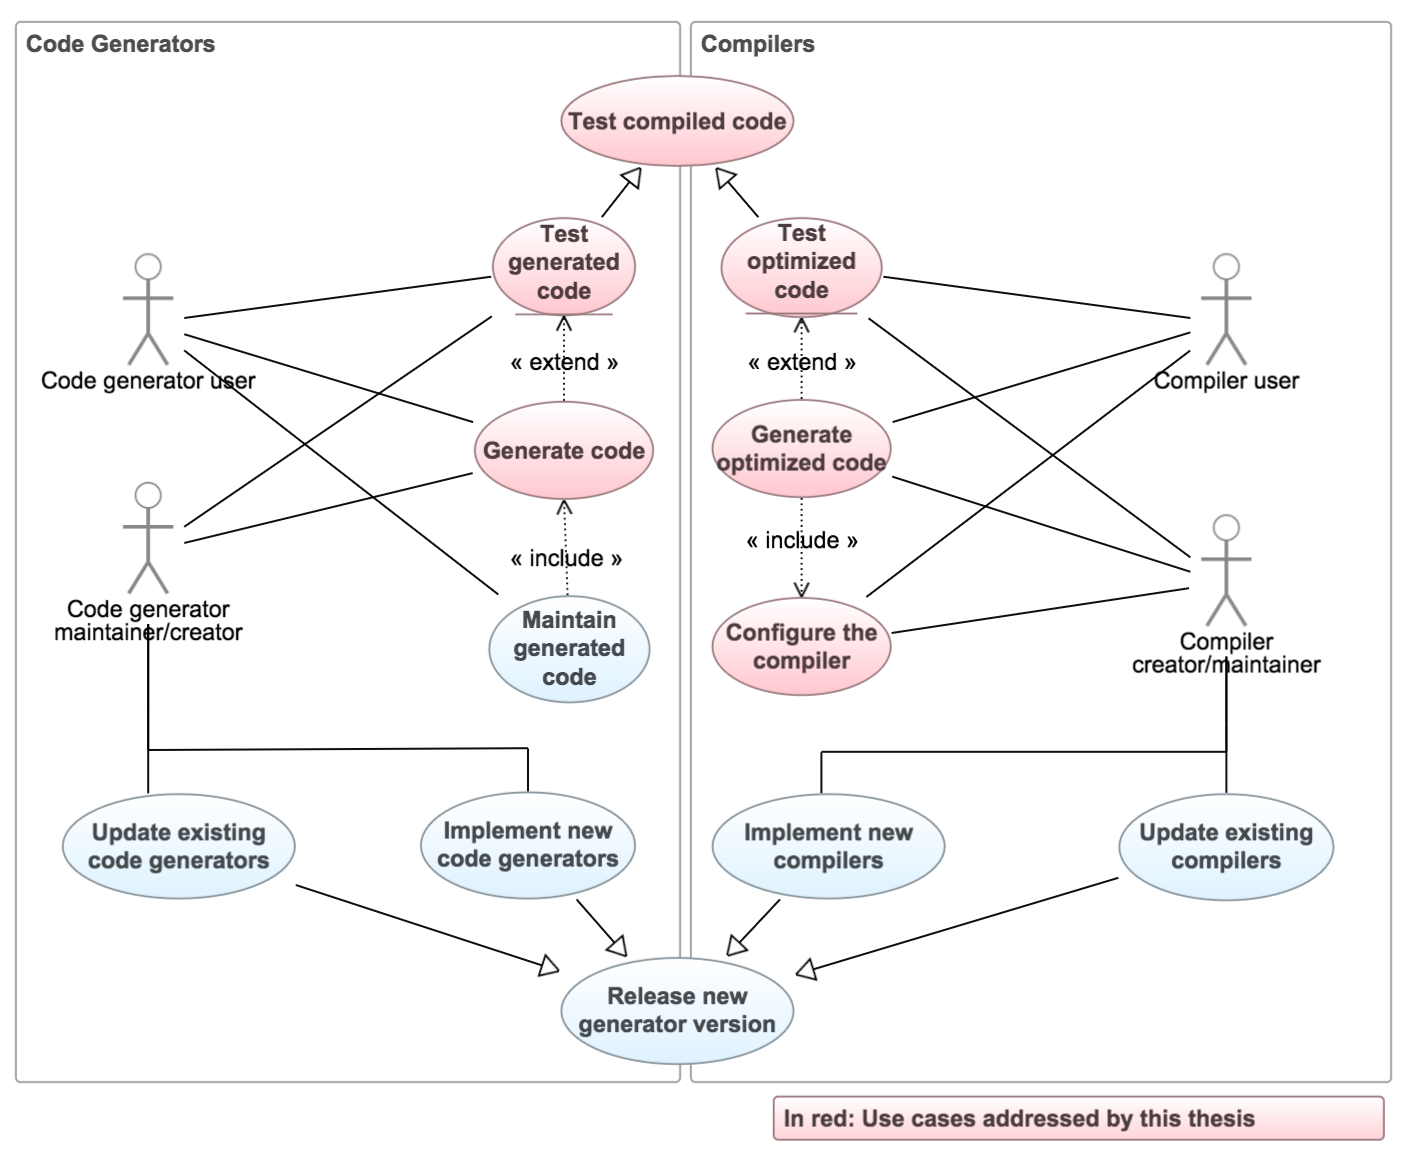
\includegraphics[scale=0.45]{Background/fig/usecase}
	\caption{Use case diagram of the different actors/roles involved in testing and tuning generators}
	\label{fig:usecase}
\end{figure}
Software development involves several stakeholders that play different roles for validating and testing the software development chain described previously.
Figure \ref{fig:usecase} depicts a use case diagram that describes these different concerns, actors and roles for testing and tuning generators.

Basically, we distinguish two stakeholders: generator user and creator/maintainer. As shown in the bottom of Figure \ref{fig:usecase}, creators/maintainers of generators are responsible of the correct functioning of generators. They use their expertise and knowledge associated to the software and hardware technologies, resulting in efficient code generation. They contribute to the software development community by creating and providing new optimizations and compiler versions updates. For code generators, they may use their knowledge to build new platform-specific code generators or enhance existing ones. 

On the other side, generator users represent the group of software developers that have no knowledge/expertise about the way code is generated. Thus, they are unable to edit or maintain the internal behavior of generators (e.g., the case of commercial and off-the-shell code generators/compilers). In this case, generators are used as black box components by engineers during software development to ease code production. Therefore, developers may configure compilers by providing the set of configuration options to efficiently produce code for the target hardware platform (e.g., optimizations options) or maintain/edit the generated code in case of automatic source code generation.

The uses cases highlighted in red in Figure \ref{fig:usecase} constitute the main tasks that we are addressing in this thesis. Our main concern is to evaluate the non-functional properties of automatically generated code.

On the one hand, we would help code generator users to test the automatically generated code and detect code generator issues by evaluating the resource usage and performance properties. This task may involve both, code generator users and creators/maintainers.

On the other hand, we would help compiler users to auto-tune compilers through the use of optimizations provided by compiler experts. Similarly, this concerns both actors and it consists in evaluating the impact of these configurations on the performance and resource usage properties and finding the best set of optimizations for a specific program and target hardware architecture.

%\begin{figure}[h]
%\center
%	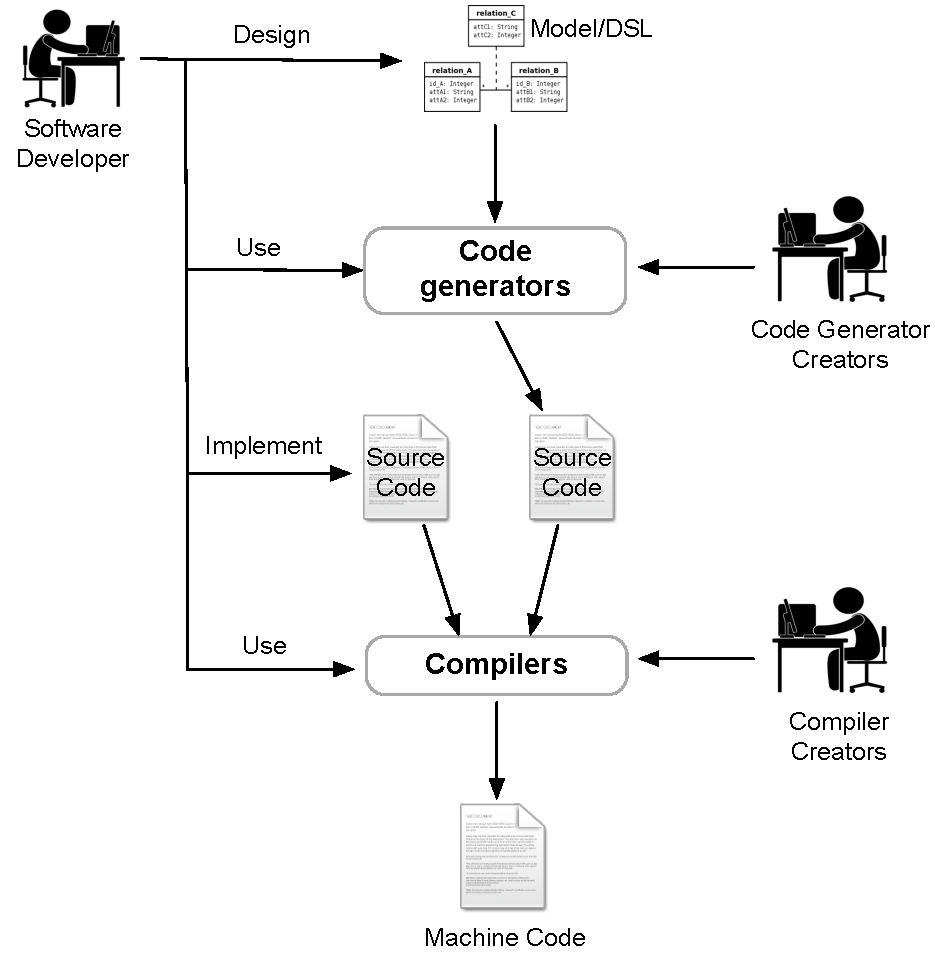
\includegraphics[scale=0.65]{Background/fig/background_overview.pdf}
%	\caption{Overview of the Docker-based testing architecture}
%\end{figure}

\section{Testing code generators}
\label{bg:Testing code generators}
In this thesis, we focus on testing the automatic code generation process (highlighted in red in the left side of Figure \ref{fig:usecase}). To do so, we introduce in this section some basis about code generators. We give an overview of the different types of code generators and we discuss their complexity which constitute a major obstacle for testing.
\subsection{Testing workflow}
The main goal of generators is to produce software systems from higher-level specifications. Generators bridge the wide gap between the high-level system description and the executable.
\begin{figure}[h]
	\center
	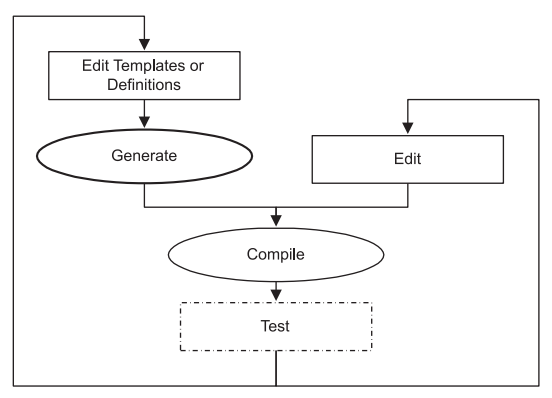
\includegraphics[scale=0.7]{Background/fig/workflow}
	\caption{Code generation workflow}
	\label{fig:workflow}
\end{figure}

As stated before, the code generation workflow is divided into two levels. It starts by transforming the system design into source code through the use of generators. Afterwards, source code is transformed into executables using compilers. Thus, software developers use to generate code, edit it (if needed), compile it and then test it. If changes are applied to compilers or generators, the cycle is repeated. Figure \ref{fig:workflow} presents an overview of this testing cycle. The right-hand side of the figure shows the classic workflow for developing and debugging code which is \textit{“edit, compile, and test.”}. The user writes or edits an existing code, compiles it using specific compilers, and tests it. Code generation adds a few new workflow elements in the left-hand side of the figure where generator creators edit the templates and definition files (or the generator itself) and then run the generator to create new output files. The output files are then compiled and the application is tested. 



\subsection{Types of code generators}
\label{bg:Types of code generators}
There are many ways to categorize generators. We can differentiate them by their complexity, by usage, or by their input/output. According to\cite{herrington2003code}, there are two main categories of automatic code generation: passive or active. Passive code generators build the code only once, then it’s up to the user to update and maintain the code. 
The most common use of passive code generators are wizards. 

Active code generators, run on code multiple times during the lifecycle. With active code generators, there is code that can be edited by the users, and code that should only be modified by the code generator. Active code generators are widely referenced in the literature\cite{pais2005tool,amanquah2009rapid}. We focus in this thesis, on testing this class of code generators.
In the literature \cite{herrington2003code,hunt2000pragmatic,fertalj2008source,bajovs2013code}, researchers define six categories of active code generators: 

\begin{itemize}
\item \textbf{Code munger:} A code munger reads code as input and then builds new code as output. This new code can either be partial or complete depending on the design of the generator.
A code munger is the most common form of code generators and are used widely. This kind of generators are often used for automatically generating documentations.
A source-to-source compiler, transcompiler or transpiler \footnote{\url{"https://en.wikipedia.org/wiki/Source-to-source_compiler"}} can also be defined as code mungers. A transcompiler takes a code written in some programming language and translates it to a code written in some other language. \textbf{Our contribution related to code generators testing will focus on this kind of generators to validate our approach for automatically detecting inconsistencies.}

Examples:  C2J, JavaDoc, Jazillian, Closure Compiler, Coccinelle, CoffeeScript, Dart, Haxe, TypeScript, and Emscripten



\item \textbf{Inline code expander:} This model reads code as input and builds new code that uses the input code as a base but has sections of the code expanded based on the design of the original code. 
It starts with designing a new language. Usually this new language is an existing language with some syntax extensions. The inline code expander is then used to turn this language into production code in a high-level language.

Example: Embedded SQL languages such as SQLJ (for Java) and Pro*C (for C). The SQL can be embedded in the C or Java code. The generator builds production C code by expanding the SQL into C code which implements the queries for example.

\item \textbf{Mixed code generator:} This model has the same processing flow as the Inline Code Expander, except that the input file is a real source file that can be compiled and run. The generated output file keep the original markup that will denote where the generated code was placed. It enables code generation for multiple small code fragments within a single file or distributed throughout multiple files. Generally, transformation rules are defined using regular expressions.


Example: Codify is a commercial mixed-code generator which can generate multiple code fragments in a single file from special commands. Another example is the replacement of comments in the input file by the corresponding code.

\item \textbf{Partial class generator:} A partial class generator takes an abstract definition as input instead of code (e.g., UML class diagram) and then builds the output code. User then, can extend it by creating derived classes and extending methods to complete the design. Turning models into code is done through a series of transformations. For example, platform-independent model (PIM) is transformed into a platform specific model (PSM). Then code generation is performed from PSM by using some sort of template-based code transformations.
%As an example, in model-driven engineering, a platform-dependent model (PIM) is transformed into a platform specific model (PSM). PIM to PSM translations are done either by hand or by applying automatic model transformation tools. Then code generation is performed from PSM by using some sort of template-based code generator.

Example: ArgoUML and Codegen translate UML class diagrams to general-purpose languages such as C\#, Java and C++. They do not generate complete implementations, but they try to convert the input UML class diagrams into skeleton code that the user can easily edit it. 

\item \textbf{Tier generator:} In this model the generator builds a complete set of output code from an abstract definition. It has the same concept as Partial class generator. The big difference between tier and partial class generation is that in the tier model the generator builds all the code for a tier. This code is meant to be used without extension. The partial-class generator model however, lets the engineer create the rest of the derived classes that will complete the functionality for the tier.

Examples: Database Access layer, Web client layer, Data export, import, or conversion layers

\item \textbf{Full-domain language:} Domain languages are basically new languages that have types, syntax and operations and they are used for a specific type of problem. 
Domain languages are the extreme end of automatic code generation because developers have to write a compiler for each problem domain and language. 

Example: Matlab is a domain specific math language that makes it easy to represent mathematical operations for example rather than object-oriented languages. DSLs are other examples such as ThingML\footnote{\url{http://thingml.org/}} and its code generators.

\end{itemize}
%Generators are based on domain-specific models which define the semantics of the system specification language and also contain the knowledge of how to produce efficient implementations[REF]. 
%We distinguish two major types of code generators: rule-based model-to-model transformation languages (such as ATL) and template-based model-to-text transformation languages (such as Acceleo) to translate high-level system specifications into executable code and scripts.
\subsection{Why testing code generators is complex?}
\label{sec:Why testing code generators is complex?}
Verifying and validating the automatic code generators raise different challenges.
In the following, we discuss major problems of code generators testing:
\begin{itemize}
	\item[--] \textbf{The oracle problem}: 
	
	To test the automatic code generation, test oracles are required to assess whether a test has passed or not. A test
	oracle checks whether the result of executing a test is as expected.
	In case of functional testing of code generators, the test oracle can be easily defined. For example, it can be defined as the comparison result between the simulated or executed model and its corresponding implementation. 
	However, in case of non-functional testing of code generators, the testing oracle is complex to define. In fact, the generated code has to meet certain performance requirements (e.g. execution speed, response time, memory consumption, utilization of resources, etc.). Proving that the generated code respects one of these non-functional requirements is not obvious. For example, one kind of solutions that can be applied is to perform a non-regression testing approach to compare the non-functional properties of two implementation versions of generated code.
	
	\item[--] \textbf{Infeasibility of unit testing}:
	 
	It is infeasible to test a whole code generator exhaustively with traditional software test approaches due to the complexity of the tool. When it comes to the unit testing of code generators, each translation function would have to be detached from the software system and surrounded by a test harness. This means decoupling each translation rule and testing it separately. This is, however, infeasible because it is difficult to address this specific functionality separately when testing a system as a whole. 
	Consider, for example, functional testing of the translation function for the sum operator (+). According to\cite{burnard2004verifying}, there are more than 2.000 ways of implementing the function a = b + c since the operation depends on data types and whether data limiting is enabled or not.
		
	\item[--] \textbf{Complexity of code generators}: 
	
	Code generators can be difficult to understand since they are typically composed of numerous elements, whose complex interdependencies pose important challenges for developers performing design, implementation, and maintenance tasks. 
	Given the complexity and heterogeneity of the technologies involved in a code generator, developers who are trying to inspect and understand the code-generation process have to deal with numerous different artifacts. As an example, in a code-generator maintenance scenario, a developer might need to find all chained model-to-model and model-to-text transformation bindings, that originate a buggy line of code to fix it. This task is error prone when done manually. So, flexible traceability tools are needed to collect and visualize information about the architecture and operational mechanics of code generators, to reduce the challenges that developers face during their life-cycle\cite{guana2015developers}. 
	Table \ref{tab:targetlink} shows, as an example, some metrics of the TargetLink code generator version 2.0. TargetLink\footnote{\url{https://www.dspace.com/en/inc/home/products/sw/pcgs/targetli.cfm}} is a software system that generates production code (C code) straight from the MATLAB/Simulink/Stateflow graphical development environment. 
	\begin{table}
		\centering
		\caption{Metrics of the TargetLink code generator}
		\begin{tabular}{| l | c | }\hline
			\textbf{Metrics} & \textbf{TargetLink code generator 2.0}  \\	\hhline{|=|=|}	
			No. of classes  & 3000\\ 
			No. of files & 6000 \\  
			No. of functions & 51.000 \\  
			Lines (total) & 1.800.000 \\  
			Lines of code & 990.000 \\ 
			Lines of comments  & 560.000 \\ 	\hline
		\end{tabular}
		\label{tab:targetlink}
	\end{table}
	This table shows how huge is the code generator base code. With more than 1.800.000 lines of code, it is very hard to test thz whole system. 
	
	\item[--] \textbf{Non-executable source model}: 
	
	Code generators do not always support executable source models. Sometimes, code generators such as partial class generator, generate only structural code through a series of transformations from a non-executable model (e.g., UML diagrams). It is up to the users next, to extend the generated code by extending the derived classes. 
	As an example, model-based code generators integrate rule-based model-to-model transformation languages to transform one model to another (such as ATL).
	In case of non-executable models, verifying that the produced code has a correct behavior as it is described in the specification model becomes difficult since it is not executable.   

	
	%The challenge is that the structure of the specification is usually very different from the structure of the implementation: there is no simple one-to-one correspondence between the concepts in the specification and the concepts in the implementation. 
\end{itemize}

%Efficient implementations are then computed at generation time by applying domain-specific optimizations and replacing, merging, adding, and removing components.

%\begin{figure}[h]
%	\center
%	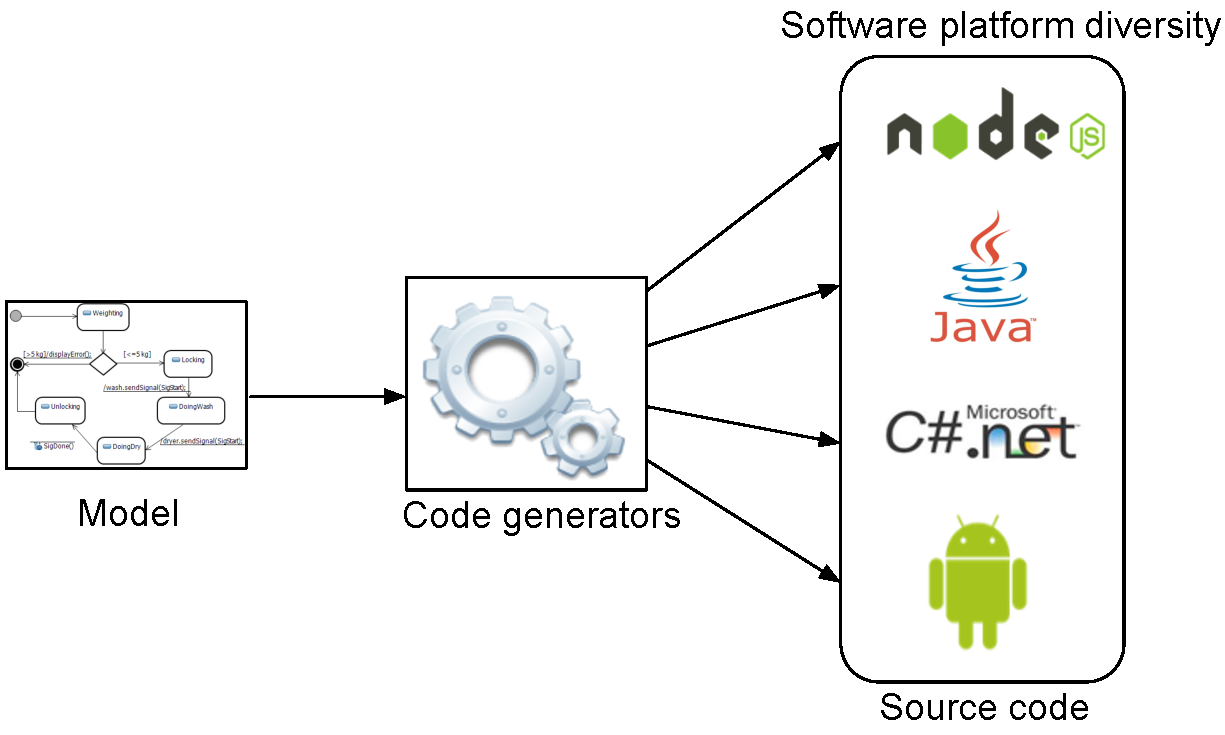
\includegraphics[scale=0.65]{Background/fig/software-diversity.pdf}
%	\caption{Code generation process}
%\end{figure}




\section{Compilers auto-tuning}
\label{bg:Compilers auto-tuning}
The compiler is a very essential software component in software engineering, responsible for translating user'source code written in general purpose languages into machine code. The key feature of compilers is to bridge source programs written in high-level languages with the underlying hardware architecture.

High-level languages are used to help the software developer to have an easier and simpler way for writing programs. They offer many abstract programming features such as functions, data structures, conditional statements and loops that facilitates software development.
Writing code in a high-level programming language may induce significant decrease in performance. Principally, software developers should write understandable, maintainable code without putting too much emphasizes on the performance for example. 

This means that the compiler has a major role in automatically producing fast and efficient target machine code. This is not a trivial task because potentially many variants of the machine code exist for the same program. Hence, the task of the compiler is to find and produce the best version of the machine code for any given program. For this reason, compilers generally attempt to automatically optimize the code to improve its performance.
This process is called code optimization. 

\subsection{Code optimization}

Code optimization within a compiler is the process of transforming a source code program into another functionally equivalent code for the purpose of improving one or more of its non-functional properties. 
The most common outcome of optimizations is to minimize the execution time of program execution. Other less common non-functional properties are code size, memory usage and power consumption. 
There exist many types of optimizations such as loop unrolling, automatic parallelization, code-block reordering and functions inlining among others. The factors that affect optimizations may include characteristics such as: the number of CPU registers (the more registers, the easier it is to optimize for performance), cache size, CPU architecture, etc.

Optimization can be categorized broadly into two types: machine independent and machine dependent: 
\begin{itemize}
	
	\item \textbf{Machine-independent optimization:}
	
	Intermediate code generation  inside compilers may introduces many inefficiencies such as extra copies of variables and using variables instead of
	constants.
	This kind of optimizations removes such inefficiencies and improves code. Thus, the compiler takes in the intermediate code and transforms a part of the code regardless of any CPU registers or memory locations. These optimizations generally change the structure of programs.
	Optimizations that are applied on abstract programming concepts (structures, loops, objects, functions) are independent of the machine targeted by the compiler.
	
	\textbf{Example:} Eliminate redundancy, loop unrolling, eliminate useless and unreachable code, function inlining, dead-code elimination, etc.
	
	\item \textbf{Machine-dependent optimization:} 
	Machine-dependent optimizations are applied after generating the target code and when the code is transformed according to the target machine architecture. They take advantage of special hardware features to produce code which is shorter or which executes more quickly on the machine such as instruction selection, register allocation, instruction scheduling, introduce parallelism, etc.
	They mostly involve CPU registers and memory references. Machine-dependent optimizers put efforts to take maximum advantage of memory hierarchy. They are more effective and have better impact on performance than independent optimizations because they best exploit special features of the target platform.
	
	\textbf{Example:} Register allocation optimizations for efficient utilization of registers, branch prediction, loop optimization, etc
 
 
\end{itemize}
 

 
 
 

\subsection{Why compilers auto-tuning is complex?}
\label{sec:Why compilers auto-tuning is complex?}
%\subsection{Why complier auto-tuning is complex?}
Today, modern compilers implement a broad number of optimizations. Each optimization tries to improve the performance of the input application.

On the one hand, optimizing compilers becomes quite sophisticated nowadays. Creating compiler optimizations for a new microprocessor is a hard and time-consuming work because it requires a comprehensive understanding of the underlying hardware architecture as well as an efficient way to evaluate the optimization impact on the non-functional properties. 

On the other hand and from the compiler user perspective, applying and evaluating optimizations is challenging because the determination of the optimal optimizations set has been identified as a major research problem in the literature\cite{knijnenburg2002iterative}.

We resume, in the following, several issues that make the activity of compiler tuning very complex:

\begin{itemize}
	\item[--] \textbf{Conflicting objectives:} Compilers usually have to support a variety of conflicting objectives, such as execution time, compilation speed, resource usage and quality of generated code. It is difficult to define a set of optimizations that satisfy all properties.
	
	\item[--] \textbf{Optimization interactions:} The interaction between optimization phases as well their application order make it difficult to find an optimal sequence.
	
	\item[--] \textbf{Huge number of optimizations:} The huge number of optimizations is also an issue for the compiler user to choose the best optimization sequence since an exhaustive search is impossible (we count $2^{number\ of\ optimizations}$ possible combination to evaluate).
	
	\item[--] \textbf{Non universal optimizations:} There is no one universal optimization sequence that will enhance the performance of all programs. Optimization's impact depends on the hardware and on the input program. Thus, constructing an optimization sequence for different programs and hardware architectures becomes very hard and time-consuming.
	
	\item[--] \textbf{Compiler bugs:} Applying optimizations may introduce errors in the compiled code and results in compiler bugs\cite{le2014compiler,yang2011finding}. Therefore, tuning compiler must not cause any change in the program behavior.
	
	\item[--] \textbf{Optimization overhead:} Optimizations should be fast and efficient. They should not delay the overall compiling process. Instead, we apply optimizations to enhance some properties, not to induce performance regressions/overhead.
	
	\item[--] \textbf{Tuning compilers need expertise:} In case the compiler user has no knowledge and expertise about the compiler technology and its optimizations, it will be quite hard to select the set of optimization sequences to apply.
\end{itemize}

 

%Improvement of source code programs in terms of performance can refer to several different non-functional properties of the produced code such as code size, resource or energy consumption, execution time, among others~\cite{almagor2004finding,pan2006fast}.
%\begin{figure}[h]
%	\center
%	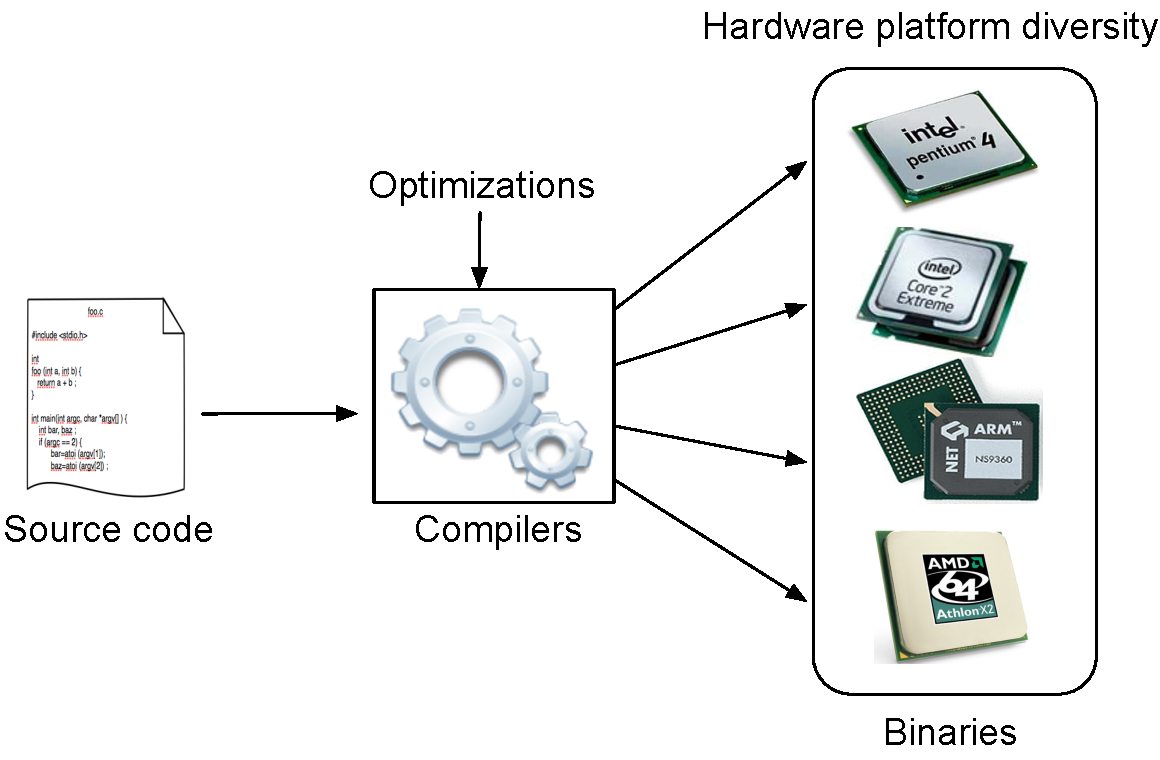
\includegraphics[scale=0.65]{Background/fig/hardware-diversity.pdf}
%	\caption{Compiler optimizations}
%\end{figure}


\section{Summary: challenges for testing and tuning configurable generators}
\label{bg:Summary: Testing and optimization challenges}
We resume in this section the main testing and tuning challenges we have identified through this chapter.
\begin{itemize}
	\item \textbf{Heterogeneous execution environments}: 
	The diversity of existing software environments and platforms as well as the hardware heterogeneity make the testing activity of generators very difficult. Deploying and executing the automatically generated software artifacts on top of a bench of platforms is time consuming. Thus, an effective mean is needed to facilitate software testing and optimization.
	\textbf{How can we leverage the new advances in software engineering technologies to face the continuous hardware and software innovation when testing/tuning generators?} 
	
    \item \textbf{The oracle problem when testing code generators}: 	
	Automatic code generation offers many gains over traditional software development methods. e.g., speed of development, increased adaptability and reliability. But code generators are complex pieces of software that may themselves contain bugs. Thus, testing code generators becomes very needed. The test oracle problem as discussed in section \ref{sec:Why testing code generators is complex?} is one of the main challenges related to the non-functional testing of code generators. This problem occurs also in functional testing, when dealing with non-executable models.
	\textbf{
	%So, how can we automatically detect issues within code generators? 
	So, proving that the generated code is functionally correct is not enough to claim the effectiveness of the code generator under test? How about the non-functional requirements such as resource consumption?
	How can we efficiently detect these non-functional code generator issues?}
	
	\item \textbf{Large optimization search space when auto-tuning compilers}: 
	Compilers may have a huge number of potential optimization combinations, making it hard and time-consuming for software developers to find/construct the sequence of optimizations that satisfies user specific key objectives and criteria. It also requires a comprehensive understanding of the available optimizations of the compiler and their interactions. Moreover, it is difficult to find the optimization sequence that represents a trade-off between two conflicting objectives.  
	\textbf{So, how can we help the compiler user to automatically tune compilers and choose the optimization that satisfy a one or two specific non-functional requirement? }
	
	\item \textbf{Monitoring the resource usage of automatically generated code:} 
	Analyzing the resource usage of optimized or generated code requires a dynamic and adaptive solution that extract efficiently those properties. Due to the software diversity and hardware heterogeneity, monitoring the resource usage of each execution platform becomes challenging and time-consuming. 	
	\textbf{So, how can we ease this process and provide an efficient solution that will help compiler users/experts to evaluate the optimizations and code generator users/experts to test the generated code in terms of resource usage?}
	

	

%\subsection{Resource usage monitoring}
\end{itemize}


%
